\section{Colorizar}

\subsection{Código C}
	El código C se trata de una conjunción de ciclos, el exterior que recorre desde la segunda fila hasta la ante última,  y el interior que recorre desde la segunda columna hasta la última, dejando afuera a todos los bordes, tal como el enunciado pedía. \\ Luego en cada iteración del ciclo interior, que es donde se hacen las opearciones que modifican la imagen, lo que hacemos es crear un arreglo de unsinged chars, "res", que es  donde guardamos los máximos de cada canal en comparación a todos  los pixeles lindantes del píxel en el cual estemos parados (una matriz de 3x3).
\begin{itemize}
\item {Res $[$0$]$ $\leftarrow$ MaximoLindantesAzul}
\item {Res $[$1$]$ $\leftarrow$ MaximoLindantesVerde}
\item {Res $[$2$]$ $\leftarrow$ MaximoLindantesRojo}
\end{itemize}
Luego con estos tres valores calculamos el alpha correspondiente de cada canal por el cual vamos a multiplicar a cada uno. Y por último reescribimos el píxel final, en la imagen src con cada canal multiplicado por dicho alpha.

\subsection{Código ASM}
	El código en ASM se trata también de una conjunción de ciclos. El ciclo exterior recorre desde la segunda hasta la ante última fila, y el interior recorre las columnas desde la segunda hasta la ante última, pero saltando de a dos píxeles, que es la cantidad que procesamos simultaneamente con instruccciones SSE. \\
	El ciclo interior consta de dos partes, la primera es calcular un registro en el que en las primeras dos DW guardamos los máximos valores de cada canal entre los píxeles lindantes, en sus posiciones respectivas. Se vería asi:\\
\ Vamos a hacer referencia como "fruta" cuando un byte tenga información que no nos interesa.
\par{\textbf{XMM1:}}
\xmmb{$Fruta$}{$Fruta$}{$Fruta$}{$Fruta$}{$Fruta$}{$Fruta$}{$Fruta$}{$Fruta$}{$A_M{p2}$}{$R_M{p2}$}{$G_M{p2}$}{$B_M{p2}$}{$A_M{p1}$}{$R_M{p1}$}{$G_M{p1}$}{$B_M{p1}$}
	
 Luego con esta información lo que hacemos es duplicar dicho registro y calcular el máximo de los máximos. Lo que hacemos para lograr esto es shiftear un byte a la derecha al registro duplicado, cosa de poder ir comparando entre ellos a los valores máximos de cada canal, y finalmente reproducimos el valor del máximo entre los máximos en todas las posiciones. El seguimiento de esta operación sería la siguiente: 
\\Vamos a utilizar para esto los registros xmm1, y xmm2
\\
\par{\textbf{XMM2:}}
\xmmb{$Fruta$}{$Fruta$}{$Fruta$}{$Fruta$}{$Fruta$}{$Fruta$}{$Fruta$}{$Fruta$}{$A_M{p2}$}{$R_M{p2}$}{$G_M{p2}$}{$B_M{p2}$}{$A_M{p1}$}{$R_M{p1}$}{$G_M{p1}$}{$B_M{p1}$}
\par{\textbf{XMM1:}}
\xmmb{$Fruta$}{$Fruta$}{$Fruta$}{$Fruta$}{$Fruta$}{$Fruta$}{$Fruta$}{$Fruta$}{$A_M{p2}$}{$R_M{p2}$}{$G_M{p2}$}{$B_M{p2}$}{$A_M{p1}$}{$R_M{p1}$}{$G_M{p1}$}{$B_M{p1}$}
\par{shifteo un byte a la derecha xmm2 y hacemos pmaxub xmm1,xmm2  máximo entre ambos)}
\par{\textbf{XMM2:}}
\xmmb{$Fruta$}{$Fruta$}{$Fruta$}{$Fruta$}{$Fruta$}{$Fruta$}{$Fruta$}{$Fruta$}{$A_M{p2}$}{$R_M{p2}$}{$G_M{p2}$}{$B_M{p2}$}{$A_M{p1}$}{$R_M{p1}$}{$G_M{p1}$}{$B_M{p1}$}

\par{\textbf{XMM1:}}
\xmmb{$Fruta$}{$Fruta$}{$Fruta$}{$Fruta$}{$Fruta$}{$Fruta$}{$Fruta$}{$Fruta$}{$Fruta$}{$Fruta$}{$RG_M{p2}$}{$Fruta$}{$Fruta$}{$Fruta$}{$RG_M{p1}$}{$Fruta$}
\par {notar que varias casillas ahora tienen mas la asignación de "fruta", y esto no es porque no sepamos que hay dentro de cada una, sino que no es información relevante a nuestras operaciones y que sera pisada si es necesario dentro de pronto}
\par{luego volvemos a shiftear y repetir la operación pmaxub xmm1,xmm2  y queda: }

\par{\textbf{XMM2:}}
\xmmb{$Fruta$}{$Fruta$}{$Fruta$}{$Fruta$}{$Fruta$}{$Fruta$}{$Fruta$}{$Fruta$}{$A_M{p2}$}{$R_M{p2}$}{$G_M{p2}$}{$B_M{p2}$}{$A_M{p1}$}{$R_M{p1}$}{$G_M{p1}$}{$B_M{p1}$}

\par{\textbf{XMM1:}}
\xmmb{$Fruta$}{$Fruta$}{$Fruta$}{$Fruta$}{$Fruta$}{$Fruta$}{$Fruta$}{$Fruta$}{$Fruta$}{$Fruta$}{$Fruta$}{$RGB_{p2}$}{$Fruta$}{$Fruta$}{$Fruta$}{{\scriptsize $RGB_{Mp1}$}}
\par{por último con la instrucción pshuf, dejamos en xmm1 un registro con los máximos de los máximos representado de esta forma: }
\par{\textbf{XMM1:}}
\xmmb{$Fruta$}{$Fruta$}{$Fruta$}{$Fruta$}{$Fruta$}{$Fruta$}{$Fruta$}{$Fruta$}{$RGB_{p2}$}{$RGB_{p2}$}{$RGB_{p2}$}{$RGB_{p2}$}{{\scriptsize $RGB_{Mp1}$}}{{\scriptsize $RGB_{Mp1}$}}{{\scriptsize $RGB_{Mp1}$}}{{\scriptsize $RGB_{Mp1}$}}


	
	
   Y en la segunda parte del código lo que queda es que a este registro con la info del máximo de los máximos, lo transformamos en un registro con un 1 en el byte donde va el canal que contiene a este máximo entre los máximos (de cada píxel). Y ceros en el resto. \\ Teniendo esto se puede apreciar en el código cómo nos armamos los alphas personalizados para cada píxel y terminamos multiplicandolos y reescribiendo ambos píxeles. \\
   Por último avanzamos nuestros currents sobre columnas en dos porque es la cantidad de píxeles que procesamos y  volvemos en caso de no haber terminado toda la fila a empezar el ciclo interior.
	
	
\subsection{Experimentación}
\subsubsection{Idea}	En la experimentación de este filtro al igual que en el resto vamos a comparar el rendimiento respecto a los ciclos de clock, que tiene la funcion colorizar en C desde -o0 a -o3 contra asm. \\ Luego el segundo experimento va a consistir en probar la influencia del jump predictor en el código.\\ Primero agragando jumps de forma que no influya el flujo del programa solo para molestar al jump predictor.  Luego vamos a correrlo tal cual está, y de a poco vamos a ir desenrollando el código. Como dijimos tiene un ciclo externo y uno interno, por lo que vamos a desenrrollar primero el interno 4 veces, despues 32 y ver que pasa.\\
Y finalmente el último experimento que vamos a hacer es aprovechar el tamaño que tiene el código y vamos a desenrrollarlo completamente, de manera que generemos un código tan grande que al correrlo no entre en la memoria cache para que el PC entonces empiece a generar Miss Hits en el momento de ir leyendo la próxima instrucción y ver qué pasa entonces.
	   
\subsubsection{Hipótesis}
	Nuestra hipotesis es que el rendimiento va a ir mejorando a medida que vayamos cambiando los programas respectivamente a como los fuimos mencionando, es decir, el más lento va a ser el código de asm molestando al jmp predictor, y el mas rápido desenrollando el codigo 32 veces. \\
	Y en el el último test, por más que desenrollemos todo el programa creemos justamente que va a ser el más lento, porque justamente el tamaño del código va a generar una gran cantidad de Miss Hits en lecturas de la siguiente instrucción, y que va a vencer la optimización generada por eliminar los controladores de flujo.	
	
\subsubsection{Resultados}

\begin{figure}[h!]
\centering
	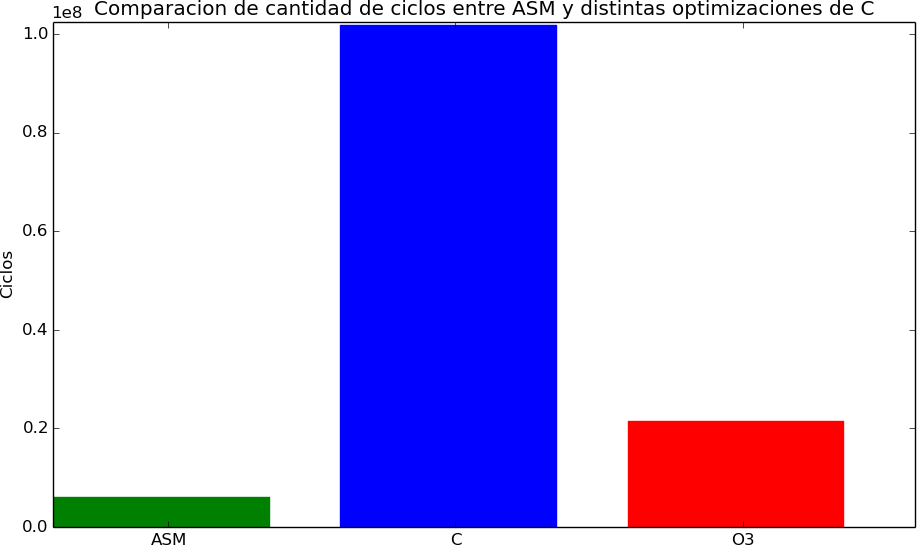
\includegraphics[width = 15 cm, height = 8 cm]{imagenes/ColorizarASMvsC.png}
	\caption[center]{Gráfico de barras comparando las implementaciones y diversas optimizaciones.}
\end{figure}

\medskip

\begin{figure}[h!]
\centering
	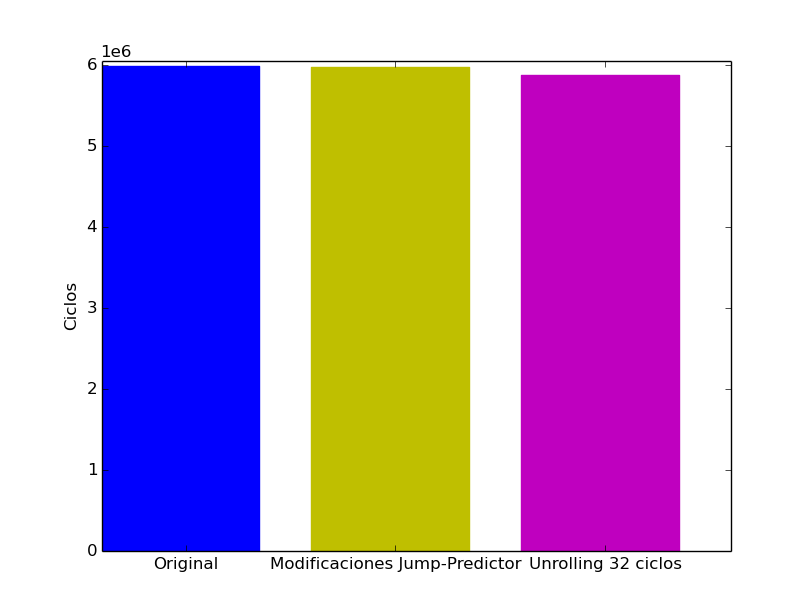
\includegraphics[width = 16 cm, height = 10 cm]{imagenes/jmpunro.png}
	\caption[center]{Gráfico de barras comparando la implementación original en ASM y la implementación en ASM con diversas modificaciones.}
\end{figure}
	
\medskip

\begin{figure}[h!]
\centering
	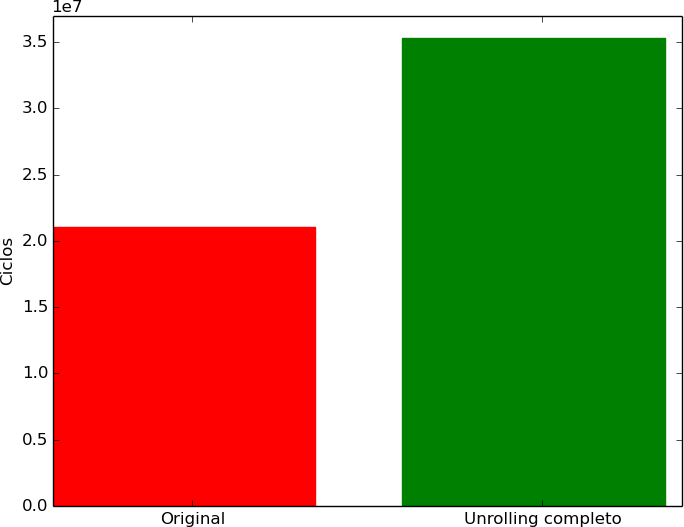
\includegraphics[width = 12 cm, height = 8 cm]{imagenes/1024.png}
	\caption[center]{Gráfico de barras comparando la implementación original en ASM y la implementación en ASM con unrolling completo aplicado a una imagen de 1024x768.}
\end{figure}
	
\subsubsection{Conclusión}
 Primera gran conclusión reveladora, c -o0 demuestra ser mucho mas lento que optimizando, el código mejoro 5 veces su cantidad de ciclos por llamada al compilar con -O3.
  Luego sin embargo la función hecha en asm le sigue ganando por bastante a C, en una proporción de 3.5 veces más rápido en cantidad de ciclos todavía.\\
  Ahora en cuanto al experimento personalizado, hicimos una comparación con distintos códigos para medir la influencia del jump predictor en la ejecución del código. Primera prueba fue la de intentar molestar al Jump Predictor. Sin embargo, por más que intentamos, descubrimos que el algoritmo que lo dirige es mucho más sofisticado de lo que pensábamos, por lo que no pudimos modificar en lo mas mínimo la eficiencia del código. \\
   Luego para contrastar el último experimento mencionado, intentamos implementar lo contrario, desenrollar el código de manera que nunca influya un Miss Jump en la ejecución del programa, sin embargo, ya con la conclusión del experimento anterior, logramos ver que desenrollar el código principal 4 y 32 veces no mostró ninguna diferencia con respecto al original. \\ 
   Por último en el experimento final con desenrollar, en el cual se pretendia desenrollar completamente el código, tuvimos mejores resultados. Funciono muy bien, lo intentamos con una imagen de 1024x768 para que el ciclo pueda ser desenrrollado más cantidad de veces, y asi se ve que el código modificado tardó en promedio al rededor de unos 14.000.00 de ciclos más que el original. Justamente por lo mencionado en la sección de hipotesis que la cantidad de Miss Hits generados por el P.C tuvo mucha mayor influencia que el tema de los jumps.
